\section{Homework 1}

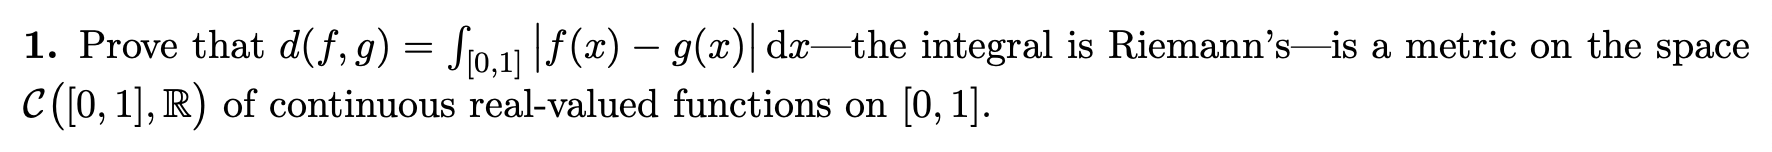
\includegraphics[width=400pt]{img/analysis--berkeley-202a--homework-1-a75a.png}

\begin{proof}
  $d$ is a metric if it satisfies (I) $d(f,f) = 0$, (II) $d(f,g) = d(g, f)$, and (III) $d(f,g) + d(g, h) \le d(f, h)$.

  (I) is satisfied: $d(f, f) = \int_{[0,1]}|f(x) - f(x)| \dx = 0$.

  (II) is satisfied:
\begin{align*}
  d(f, g)
  &= \int_{[0,1]}|f(x) - g(x)| \dx \\
  &= \int_{[0,1]}|g(x) - f(x)| \dx \\
  &= d(g, f),
\end{align*}

  (III) is satisfied:
\begin{align*}
  d(f, g) + d(g, h)
  &= \int_{[0,1]} |f(x) - g(x)| \dx + \int_{[0,1]} |g(x) - h(x)| \dx \\
  &= \int_{[0,1]} |f(x) - g(x)| + |g(x) - h(x)| \dx \\
  &\le \int_{[0,1]} |f(x) - g(x) + g(x) - h(x)| \dx \\
  &= \int_{[0,1]} |f(x) - h(x)| \dx \\
  &= d(f, h).
\end{align*}
\end{proof}

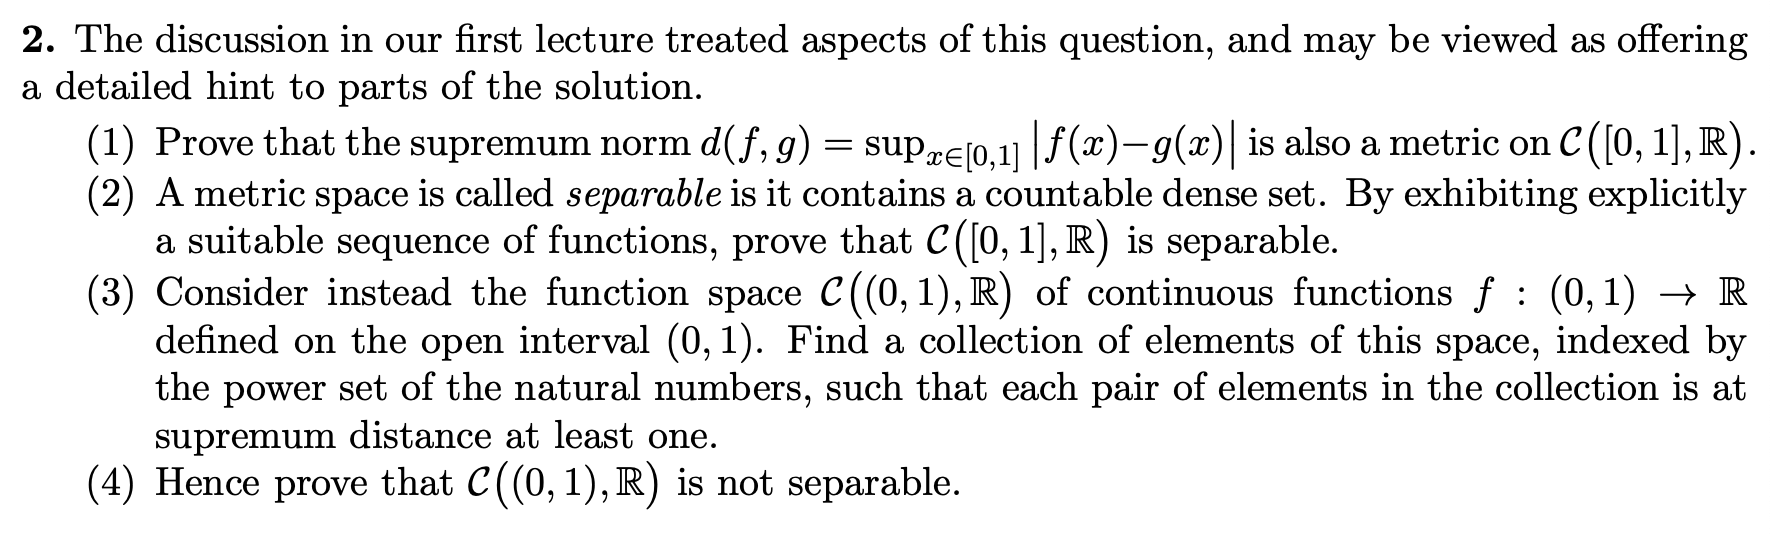
\includegraphics[width=400pt]{img/analysis--berkeley-202a--homework-1-d1d3.png}
\begin{enumerate}
\item
  \begin{proof}
    $d$ is a metric on the function space $\mathcal C\([0, 1], \R\)$ if it satisfies (I) $d(f,f) = 0$,
    (II) $d(f,g) = d(g, f)$, and (III) $d(f,g) + d(g, h) \le d(f, h)$.

  (I) is satisfied: $\sup_{x\in [0,1]} |f(x) - f(x)| = \sup_{x\in [0,1]} 0 = 0$.

  (II) is satisfied:
\begin{align*}
  d(f, g)
  &= \sup_{x \in [0,1]}|f(x) - g(x)| \\
  &= \sup_{x \in [0,1]}|g(x) - f(x)| \\
  &= d(g, f),
\end{align*}
  (III) is satisfied:
\begin{align*}
  d(f, g) + d(g, h)
  &=   \sup_{x \in [0,1]} |f(x) - g(x)| + \sup_{x \in [0,1]} |g(x) - h(x)| \\
  &=   \sup_{x \in [0,1]} \Big(|f(x) - g(x)| + |g(x) - h(x)|\Big) \\
  &\le \sup_{x \in [0,1]} |f(x) - h(x)| \\
  &=   d(f, h).
\end{align*}
  \end{proof}

\item
  \begin{claim}
    $\mathcal C\([0, 1], \R\)$ is separable.
  \end{claim}

  \begin{proof}
    Let $\mathcal F$ be the following set of piecewise affine functions: for all $N \in \N$ and for
    all $q_1, \ldots, q_N \in \Q$ then $f_{q_1, \ldots, q_N}$ is the function formed by joining the
    points $\{(0, q_1), (1/(N-1), q_2), \ldots, (1, q_N)\}$with straight lines.

    We need to \red{show that this set of functions is countable}.

    And we need to \red{show that the set is dense} in $\mathcal C\([0, 1], \R\)$.

    Define $d(f, g)$ to be the supremum distance between functions $f: [0,1] \to \R$ and $g [0,1] \to \R$.

    Let $g$ be an arbitrary function in $\mathcal C\([0, 1], \R\) \setminus \mathcal F$ and fix $\epsilon > 0$.
    We need to show that there exists $f \in \mathcal F$ such that $d(f, g) < \epsilon$. We construct such
    an $f$ using the following algorithm:

    \red{I think the basic idea here is to use the fact that the interval is closed and therefore the target
      function has extrema, so keep drawing lines to the extrema and subdividing; something like that}

    \begin{enumerate}
    \item Set $f$ equal to the function whose graph is a straight line joining $(0, g(0))$ and $(1, g(1))$. In
      other words, set $f$ such that $f(x) = xg(0) + (1-x)g(1)$.
    \item If $d(f, g) < \epsilon$, stop.
    \item Otherwise, divide the interval in half, and repeat the approximation in each half.
    \end{enumerate}
    We need to show that this algorithm terminates.


  \end{proof}

  We must exhibit a sequence of functions that is a dense and countable subset of $\mathcal C\([0, 1], \R\)$
  under the supremum norm.

  This means that for an arbitrary continuous function $g$, and for any $\epsilon > 0$, we must be able to
  construct a function that lies within $\epsilon$ of $g$.

  https://en.wikipedia.org/wiki/Piecewise_linear_function

  \begin{quote}
    A piecewise linear function is a function defined on a (possibly unbounded) interval of real numbers,
    such that there is a collection of intervals on each of which the function is an affine function. If the
    domain of the function is compact, there needs to be a finite collection of such intervals; if the domain
    is not compact, it may either be required to be finite or to be locally finite in the reals.
  \end{quote}

  \begin{definition}
    A subset $X$ of a metric space is \defn{open} if for any point $x \in X$, there exists $\epsilon$ such that a ball
    of radius $\epsilon$ centred at $x$ is a subset of $X$.

    A subset $X$ of a metric space is \defn{closed} if it is the complement of an open subset of $X$.

    (Theorem: a set $X^C$ is closed iff it contains all its limit points, i.e. every convergent sequence
    in $X^C$ has its limit in $X^C$.)

    A subset $X$ of a metric space $Y$ is \defn{dense} if every point $y \in Y$ is either in $X$ or arbitrarily close to
    a point in $X$.
  \end{definition}

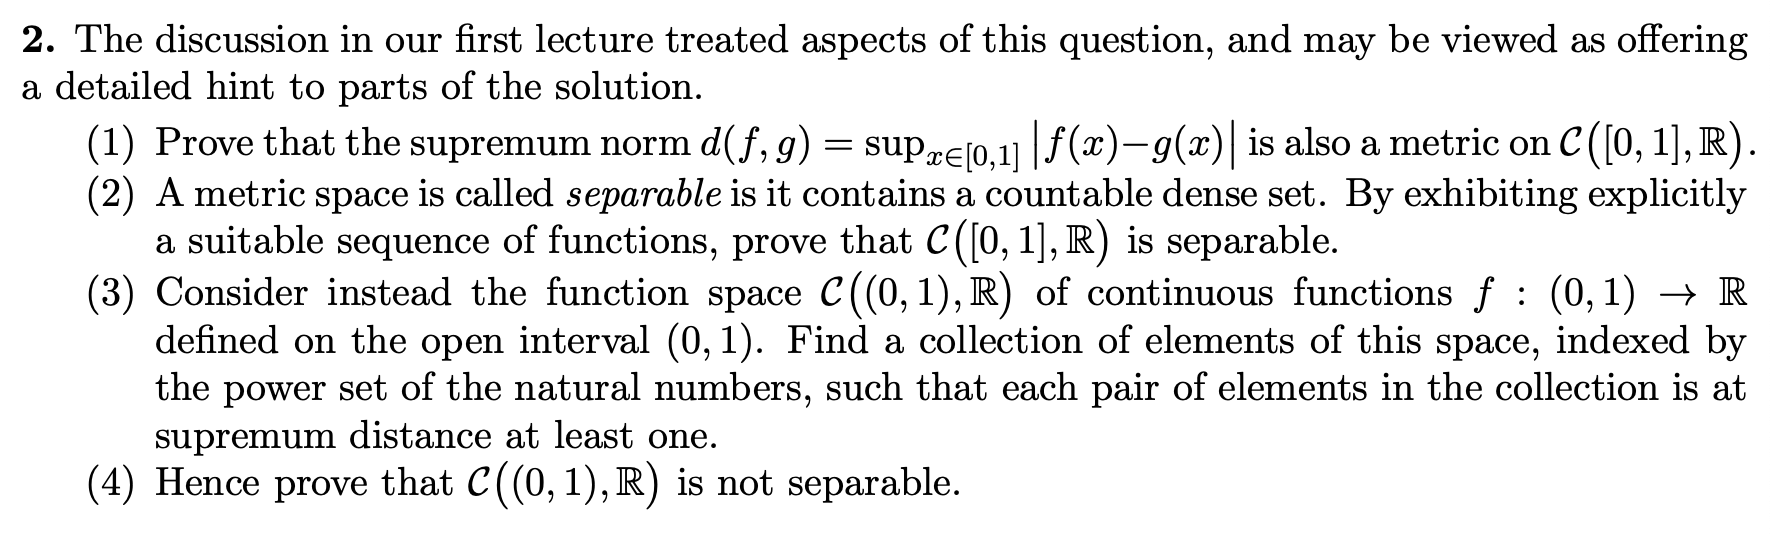
\includegraphics[width=400pt]{img/analysis--berkeley-202a--homework-1-d1d3.png}

\item Hm. Each function could be zero everywhere except a spike of height 1 at a different location from all
  other functions. But how do you make that be both continuous and yet ``narrow enough​'' for the set to have
  the same cardinality as the reals?

  Powerset of $\N$
  000...
  001...
  010...
  011...
  100...
  101...
  110...
  111...




\end{enumerate}



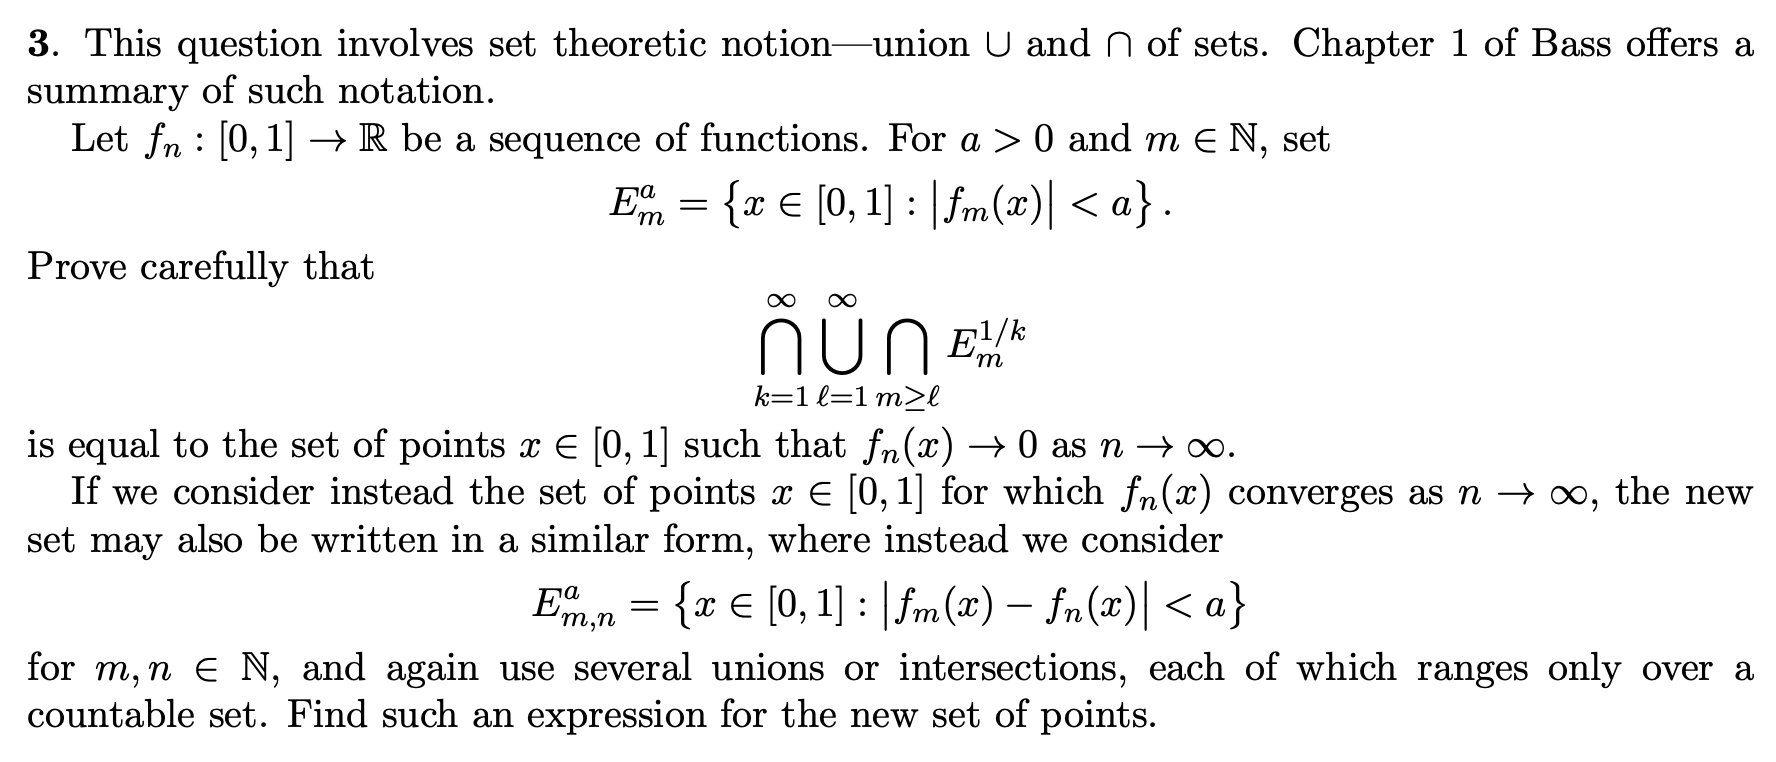
\includegraphics[width=400pt]{img/analysis--berkeley-202a--homework-1-8349.png}

\begin{proof}
  Let $E_m^a = \{x \in [0, 1] : |f_m(x) < a|\}$ and let $T = \bigcap_{k=1}^\infty \bigcup_{l=1}^\infty \bigcap_{m > l} E_m^{1/k}$.

  Informally, $E_m^a$ is the set of points for which $f_m$ is within $a$ of zero.

  Let $f_n: [0, 1] \to \R$ be a sequence of functions and let $S \subseteq [0, 1]$ be the set of points $x$
  such that $f_n(x) \to 0$ as $n \to \infty$.

  First we prove that $x \in S \implies x \in T$.

  So let $x \in S$. Then from the definition of limit we have
  \begin{align*}
    &\forall \epsilon>0 ~~~~ \exists l \in \N ~~~~ \forall m \geq l ~~~~  x \in E_m^\epsilon \\
    &\forall \epsilon>0 ~~~~ \exists l \in \N ~~~~                        x \in \bigcap_{m \geq l} E_m^\epsilon \\
    &\forall \epsilon>0 ~~~~                                              x \in \bigcup_{l=1}^\infty \bigcap_{m \geq l} E_m^\epsilon \\
    &                                                              x \in \bigcap_{k=1}^\infty \bigcup_{l=1}^\infty \bigcap_{m \geq l} E_m^{1/k} = T,
  \end{align*}
  as required.

  Secondly we prove that $x \in T \implies x \in S$.

  So let $x \in T$. We have
  \begin{align*}
    x \in \bigcap_{k=1}^\infty \bigcup_{l=1}^\infty \bigcap_{m \geq l} E_m^{1/k},
  \end{align*}
  which is equivalent to the statement
  \begin{align*}
    \forall k>0 ~~~~ \exists l \in \N ~~~~ \forall m \geq l ~~~~  |f_m(x)| < \frac{1}{k}.
  \end{align*}
  Let $\epsilon > 0$ be a real number. Then there exists $k \in \N$ such that $\frac{1}{k} < \epsilon$. Therefore we have
  \begin{align*}
    \forall \epsilon>0 ~~~~ \exists l \in \N ~~~~ \forall m \geq l ~~~~  |f_m(x)| < \epsilon
  \end{align*}
  which is equivalent to $x \in S$, as required.
\end{proof}

\begin{proof}
  Let $S \subseteq [0, 1]$ be the set of points $x$ for which $f_n(x)$ converges as $n \to \infty$. Since every
  convergent sequence in the reals is Cauchy, we have that $x \in S$ is equivalent to
  \begin{align*}
    \forall \epsilon > 0 ~~~~ \exists l \in \N ~~~~ \forall m \geq l ~~~~ \forall n \geq l ~~~~ |f_m(x) - f_n(x)| < \epsilon,
  \end{align*}
  which is equivalent to
  \begin{align*}
    \forall \epsilon > 0 ~~~~ x \in \bigcup_{l=1}^\infty \bigcap_{m \geq l} \bigcap_{n \geq l} E_{m,n}^\epsilon.
  \end{align*}
  Therefore, we have that $x \in S$ implies
  \begin{align*}
    x \in \bigcap_{k=1}^\infty \bigcup_{l=1}^\infty \bigcap_{m \geq l} \bigcap_{n \geq l} E_{m,n}^{1/k}.
  \end{align*}
  As before, the reverse implication also holds since, for any given $\epsilon > 0$ we can find a $k \in \N$
  such that $\frac{1}{k} < \epsilon$.
\end{proof}



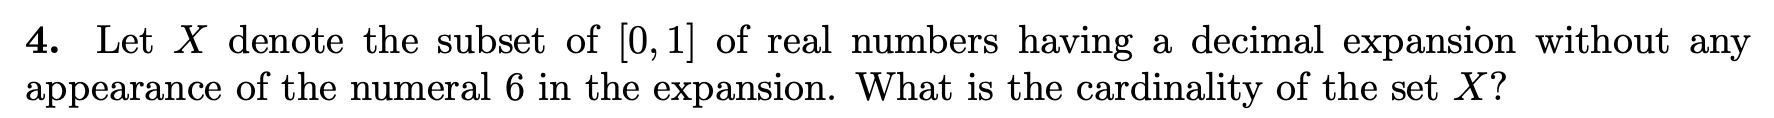
\includegraphics[width=400pt]{img/analysis--berkeley-202a--homework-1-f175.png}

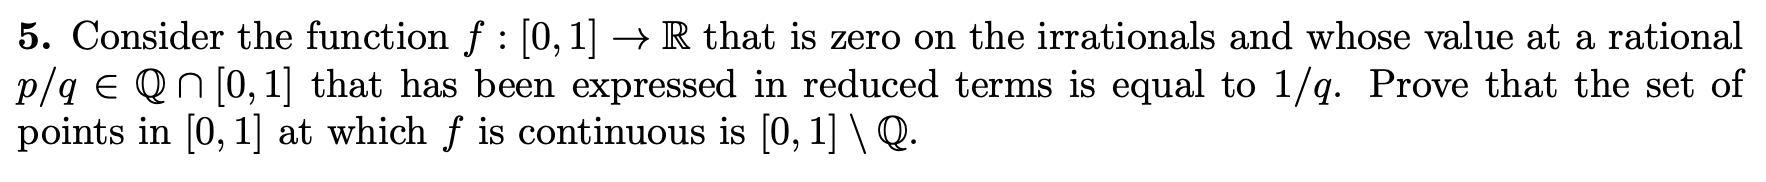
\includegraphics[width=400pt]{img/analysis--berkeley-202a--homework-1-5192.png}

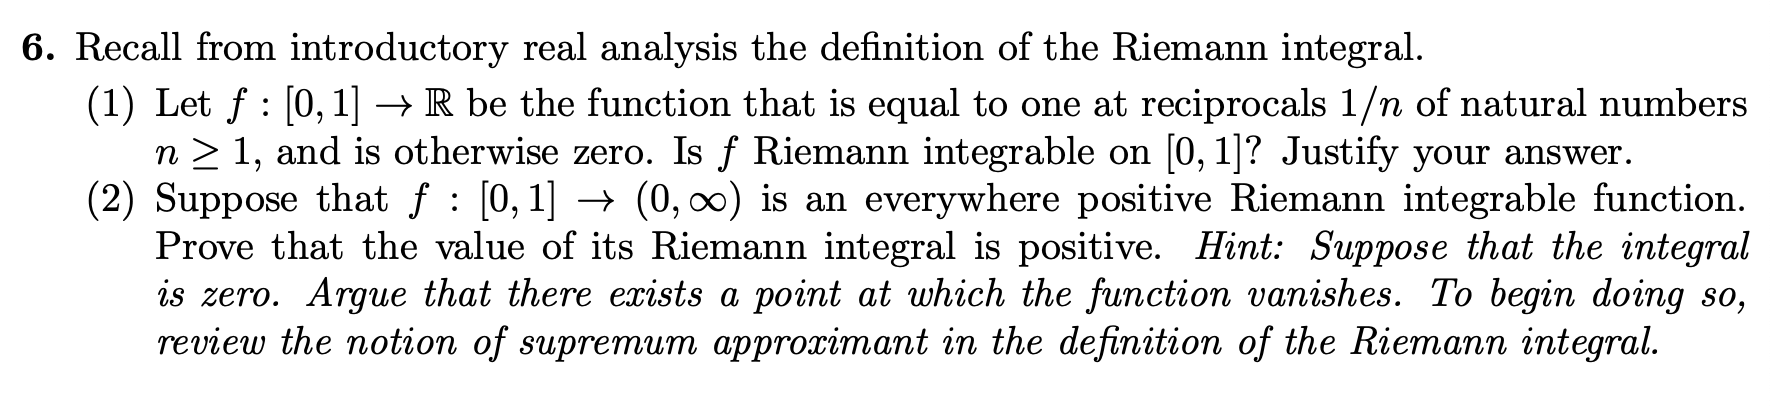
\includegraphics[width=400pt]{img/analysis--berkeley-202a--homework-1-f5e8.png}


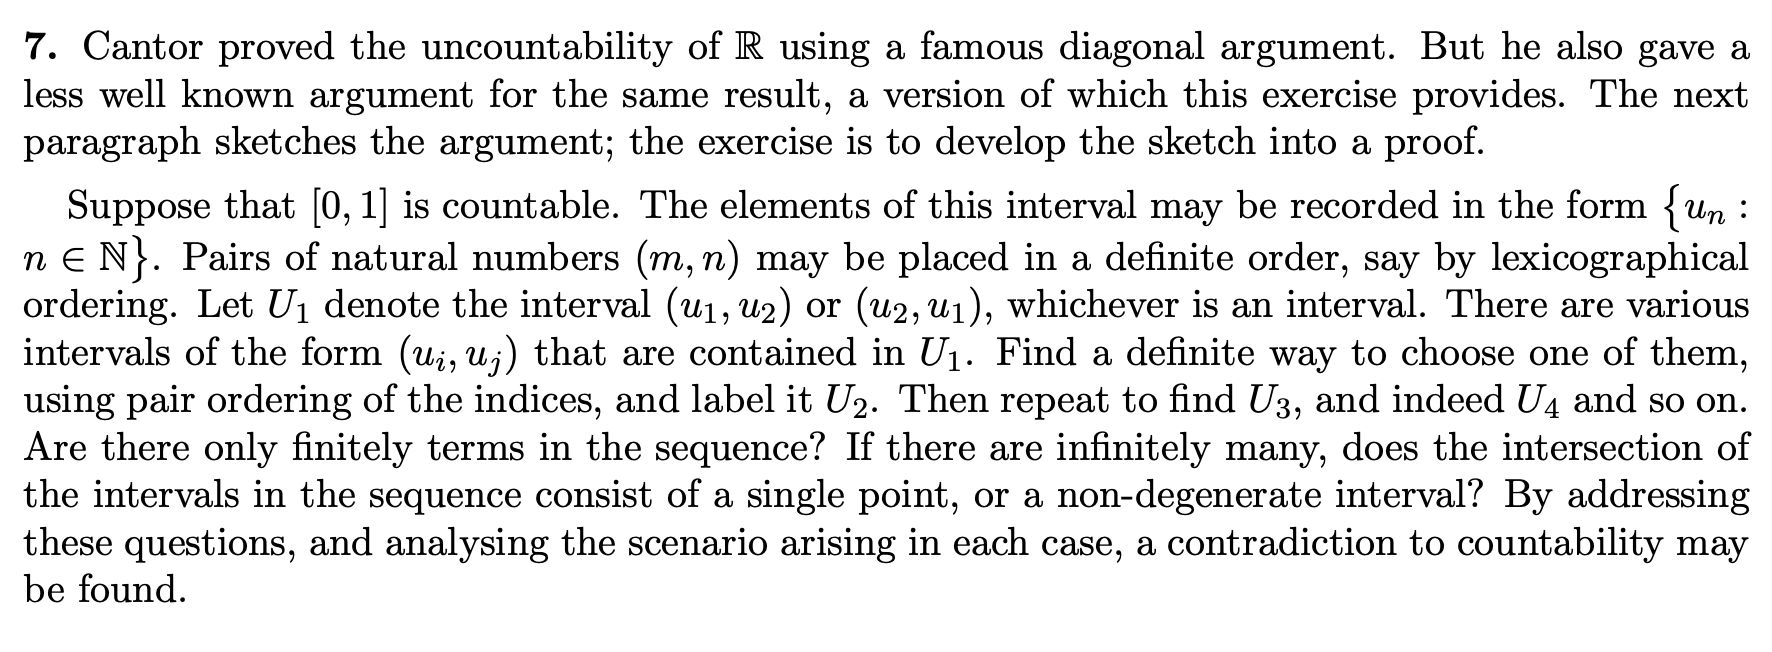
\includegraphics[width=400pt]{img/analysis--berkeley-202a--homework-1-a577.png}
